\documentclass[a4paper,english]{article}
\usepackage[utf8]{inputenc}
\usepackage[T1]{fontenc,url}
\usepackage{graphicx}
\usepackage{amsmath}
\usepackage{mathtools}
\usepackage{babel,textcomp}
\usepackage{enumitem}
\usepackage{upgreek}
\usepackage{gensymb}
\usepackage{emptypage}
\usepackage{braket}
\usepackage[version=4]{mhchem}
\usepackage{float}
\usepackage[square,numbers,comma,sort&compress]{natbib}
\bibliographystyle{unsrtnat}
\usepackage[caption = false]{subfig}
\usepackage[section]{placeins}
\usepackage{hyperref}
\usepackage[nottoc]{tocbibind}
\newcommand*{\doi}[1]{\href{http://dx.doi.org/#1}{doi: #1}} % Add Doi to link


\urlstyle{sf}

\title{The TALYS reaction code and a study of the \ce{^{153}Sm}(n,$\gamma$)\ce{^{154}Sm} reaction}
\author{Kristine Sønstevold Beckmann\footnote{In collaboration with Line G.Pedersen}}
\begin{document}

\maketitle
\section{Introduction to TALYS}
TALYS is a computer code program created to be used as a tool for physicists interested in nuclear properties. It combines theoretical modeling with the opportunity for experimental analysis.\cite{manual} By taking input in form of target nucleus, projectile and incident energy, TALYS can calculate predictions for many different reaction channels, i.e. their cross section, spectra and angular distribution. 

TALYS calculates the final cross sections using the Hauser-Feshback statistical model\cite{Goriely2008}, and includes the pre-equilibrium reaction model unlike other available reaction rate codes. TALYS can implement different available experimental data and/or several nuclear models. These models and data include nuclear masses, the optical potential, the compound nucleus, nuclear level densities and the $\gamma$-ray strength function. 

TALYS has several limitation that a user must be aware of before implementing the code in their work. One of the most significant limitation is calculations done in the resonance region of the nuclei. Since TALYS is based on the HF-model, the underlying assumption is that we are not operating with discrete levels, and therefore TALYS will not reproduce accurate results in the resonance region. It's also crucial to note that when the regions beyond experimentally known data is reached, we can not verify the models used. This leads to high uncertainties in the calculated data.

This report will look further into two of the nuclear data inputs into TALYS, namely the different level density models and compound nucleus reactions. Finally, the case of the \ce{^{153}Sm}(n,$\gamma$)\ce{^{154}Sm} reaction will be studied.
\section{Level density models}
Each nuclei have a unique set of accessible energy states they can be excited to, the structure of which depends on different nuclear properties. At low energies we most often have discrete levels, but as the excitation energy increases the levels become closer and at a certain point they will overlap, and finally they will overlap continuously. We categories these three regions as the discrete, the quasi-continuum and the continuum. The number of states at a given excitation energy, within a certain energy bin, is called the nuclear level density. Level densities are average properties of the quasi-continuum and continuum.

Reaching the quasi-continuum, which is above 2-4 MeV, you can no longer easily determine individual levels experimentally and we need methods like e.g. the Oslo Method \cite{Schiller2000} to determine level densities. We can also use different models to predict level densities. In TALYS, 6 different level density models can be implemented, 3 phenomenological models and 3 semi-microscopic models.  

The first level density model, which is the default model in TALYS, is the Fermi Gas Model combined with the Constant Temperature Model for low energies. The Fermi Gas Model was proposed by H.A. Bethe in 1936\cite{Bethe1936}, and based on the theory of Fermi statistics. Bethe proposed the idea of the nucleus as a gas consisting of non-interacting fermions. From Fermi statistics he then obtained a level density function for excitation energy $E$;
\begin{align*}
\rho{(E)} =& \frac{\sqrt{\pi}}{12}\frac{\mathrm{exp}(2\sqrt{aE})}{a^{1/4}E^{5/4}},
\end{align*} 
with the level density parameter $a$. It's predicted in this expression that the level density increases exponentially with $\sqrt{aE}$. In testing the Bethe expression this has been confirmed to be qualitatively correct, however the expression does not account for effects like pairing, collectivity and shell effects.

For modeling across the energy range in TALYS the Fermi Gas Model is combined with the Constant Temperature Model for the lower energies. The Constant Temperature Model was introduced by A.Gilbert and A.G.W.Cameron in 1965\cite{Gilbert1965}. The model is based on the assumption, extrapolated from experimental studies, that for excitation energy up to 10 MeV the total number of discrete levels can be reproduced by:

\begin{align*}
N(E) =& \mathrm{exp}(\frac{E-E_{0}}{T}),
\end{align*} 
where $T$ is the nuclear temperature and $E_0$ is the energy-shift parameter. This yields a total level density
\begin{align*}
\rho{(E)} =& \frac{dN(E)}{dE} = \frac{1}{T}\mathrm{exp}(\frac{E-E_{0}}{T}).
\end{align*} 

The second level density model used in TALYS is the Back-Shifted Fermi Gas model\cite{Dilg1973}, where the energy shift and level-density parameter are free parameters and the Bethe expression is applied to the low energies as well. This yields the expression
\begin{align*}
\rho{(E)} =& \frac{1}{\sqrt{2\pi}\sigma}\frac{\sqrt{\pi}}{12}\frac{\mathrm{exp}(2\sqrt{aU})}{a^{1/4}U^{5/4}},
\end{align*} 
for the total level density where $U=E-\Delta$ and $\Delta$ is the parameter associated with pairing energy. 

The third phenomenological level density model one can implement in TALYS is the Generalized Superfluid Model\cite{Ignatyuk1993} which is based on Bardeen-Cooper-Schrieffer theory and considers the important role superconductive pairing correlations plays in determining level densities. This model, like the first model presented, describes level densities at high excitation energies by the Fermi Gas Model. At low energies pairing correlations affect level density to a high extent and is here described with superfluid behaviour. 

The last three level density models that are available for implementation in TALYS are semi-microscopic models based on calculations done by S.Goriely and S.Hilarie \cite{manual}. The fourth level density model employs Hartree-Fock calculations done by S. Goriely up to 150 MeV in excitation energy. The fifth model proposed by S.Goriely and S.Hilaire, are calculations done based on the deformed Skyrme-Hartree-Fock-Bogolyubov. This results in a model which includes level densities dependening on spin, energy and parity. The sixth and last model uses the Gogny force in temperature-dependent Hartree-Fock-Bogolyubov calculations.

\section{Compound nucleus reactions}
We can separate nuclear reactions into three categories depending on the time lapse of the reaction, i.e. direct, pre-equilibrium and compound reactions.  For the instances with short reaction times($\sim{10^{-22}}$s) there is only a small probability for inelastic scattering and the exit channel is highly dependent on the entrance channel. This is classified as direct reactions.

Pre-equilibrium reactions takes place in the intermediate time scale between direct reactions and compound nucleus reactions. Here the projectile can react with several nucleons, but the energy of the projectile does not have time to come to equilibrium with the target nucleus. 

Compound nucleus reactions takes place where the reaction time is on such a long time scale ($\sim{10^{-17}}$s) that the projectile can react with several nucleons, and the energy of the incident particle will distribute evenly in the target and come to equilibrium. The resulting compound nucleus is then in an excited state corresponding to the kinetic energy of the projectile and binding energy. An important property of the compound nucleus reaction is that the exit channel is independent of the entrance channel in all cases except the elastic case.

Compound nucleus reactions are usually separated in to two categories when discussed. The first is the binary reaction where the projectile hits the target, the nucleus equilibriates and the resulting excited nucleus emits $\gamma$ or a particle. The second is when the the residual nucleus after a binary compound nucleus reaction remains highly excited and a process of multiple emission takes place.

For the low energy compound reaction it is needed to consider width fluctuation corrections, which means finding a factor to correct for the enhanced elastic channel. The enhancement stems from correlations between the incident and outgoing particle waves. This leads to a non-isotropic angular distribution at these low energies.

\section{Nuclear capture rates of \ce{^{153}Sm}}
The samarium isotopic chain is of great interest to nuclear physics and astrophysics. The progress of the rapid neutron capture along the chain, known as the r-process, is as of yet undetermined and missing data points. In this report the neutron capture rate and Maxwellian-Averaged cross section of \ce{^{153}Sm} at the thermal energy will be investigated. To highlight the concepts discussed in previous sections, different level density models have been implemented to show the theoretical uncertainties of TALYS calculations.

As there exists little to none available experimental data for the \ce{^{153}Sm}(n,$\gamma$)\ce{^{154}Sm} reaction, a comparison with the JEFF-3.2 library has been done. It is not unlikely that points from this evaluated library stems from TALYS itself, since no other information is available. But in that case it is interesting to see what theoretical model has been deemed most reliable by the Nuclear Energy Agency.
In \autoref{meanenergy252Cf} the spread of the cross sections according to the level densities models used is plotted. The plot confirms the above mentioned limitation of TALYS in the resonance region. And it can be seen that the evaluated data from NEA closely follows the three semi-microscopic models along most of the energy range.
\begin{figure}[H]
  \centering
      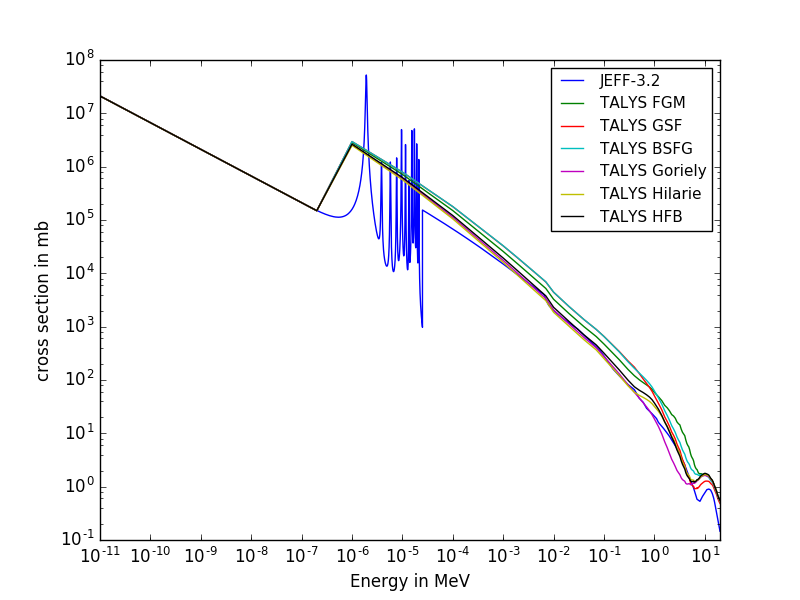
\includegraphics[width=1\textwidth]{figure_1}
  \caption{Neutron capture cross section of \ce{^{153}Sm}}
  \label{meanenergy252Cf}
\end{figure}
In addition, The Maxwellian-Averaged cross section at the thermal energy E=30 keV, is calculated and tabulated in \autoref{csvaries}. For comparison, the experimental MACS from KADoNiS\cite{kadonis} is also tabulated. It shows a clear difference from the phenomenological models to the semi-microscopic ones. The semi-microscopic values seem to fall closer to the experimental one, and this can indicate that one of these might be preferable to implement in this case.
 

\begin{table}[H]
  \centering
  \renewcommand{\arraystretch}{1.25}
    \begin{tabular}{ c c }
    \hline
    Level Density Model & MACS(mb) \\ 
    \hline
    Experimental(KADoNiS)\cite{kadonis} & 1095$\pm{175}$ \\
	Fermi Gas Model & 1406.27\\
	Back-Shifted Fermi Gas Model & 1899.10 \\
	Generalized Superfluid Model & 1892.65 \\
	Microscopic, using Gorielys tables & 890.45 \\
	Microscopic, using Hilaries tables & 811.55 \\
	Microscopic HFB & 999 \\
	\hline
    \end{tabular}
  \caption{Maxwellian-Averaged Cross Section at thermal energy E=30keV}
  \label{csvaries}
\end{table}
\section{Discussion}
In this report it has been discussed how to model and calculate nuclear cross sections using the computer code TALYS. The code aims to account for the many factors going into cross section calculations and a user must be aware of the multitude of different models and parameters included in TALYS, as well as the codes limitations.

In the case study of \ce{^{153}Sm}, it was shown how the results of the calculations can fluctuate by changing only one of the models going into TALYS, namely the level density model. From \autoref{csvaries} a clear distinction between the phenomenological and the semi-microscopic level density models is evident. It would seem in this case that the semi-microscopic models are more aligned with the experimental, and that perhaps the HFB model could be recommended as the best fit. As the semi-microscopic models aim to be based on physical theory, not only observations, this result indicates the advantages of that approach. 

This also illustrates the importance of doing calculations with the different models in TALYS and presenting theoretical uncertainties in data.
\bibliography{bobcat}
\end{document}